\documentclass[tikz]{standalone}
\usepackage{amsmath,chemformula}
\definecolor{Gold}{rgb}{1,.844,0}
\definecolor{Silver}{rgb}{.752,.752,.752}
\begin{document}
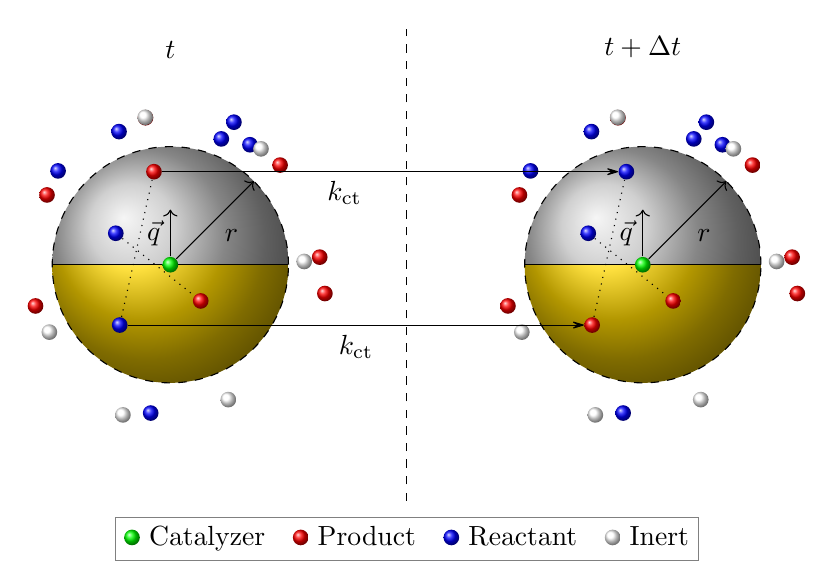
\begin{tikzpicture}[
  chemarrow,
  particle/.style = {shade,ball color=#1,circle,inner sep=2pt},
  catalyzer/.style = {particle=green},
  reactant/.style = {particle=blue},
  product/.style = {particle=red},
  inert/.style = {particle=white}
  ]
  \begin{scope}
    \begin{scope}
      \clip (-1.5,0) rectangle (1.5,1.5);
      \shade[ball color=Silver] (0,0) circle (1.5);
    \end{scope}
    \begin{scope}
      \clip (-1.5,0) rectangle (1.5,-1.5);
      \shade[ball color=Gold] (0,0) circle (1.5);
    \end{scope}
    \draw[dashed] (0,0) circle (1.5);
    \draw (-1.5,0) -- (1.5,0);
    %
    \node[catalyzer] (C1) at (0,0) {};
    \draw[->] (C1) -- node[left] {$\vec q$} +(0,.7);
    \draw[->] (C1) -- node[below right] {$r$} (45:1.5);
    \node[reactant] (R1) at (-130:1) {};
    \node[product]  (R2) at (100:1.2) {};
    \node[reactant] (R3) at (150:0.8) {};
    \node[product]  (R4) at (-50:0.6) {};
    \pgfmathsetseed{13}
    \foreach \i in {0,...,5} {
      \node[inert] at ({360*rnd}:{random(17,20)/10}) {};
      \node[reactant] at ({360*rnd}:{random(17,20)/10}) {};
      \node[product] at ({360*rnd}:{random(17,20)/10}) {};
    }
  \end{scope}
  \begin{scope}[shift={(6,0)}]
    \begin{scope}
      \clip (-1.5,0) rectangle (1.5,1.5);
      \shade[ball color=Silver] (0,0) circle (1.5);
    \end{scope}
    \begin{scope}
      \clip (-1.5,0) rectangle (1.5,-1.5);
      \shade[ball color=Gold] (0,0) circle (1.5);
    \end{scope}
    \draw[dashed] (0,0) circle (1.5);
    \draw (-1.5,0) -- (1.5,0);
    %
    \node[catalyzer] (C2) at (0,0) {};
    \draw[->] (C2) -- node[left] {$\vec q$} +(0,.7);
    \draw[->] (C2) -- node[below right] {$r$} (45:1.5);
    \node[product]  (P1) at (-130:1) {};
    \node[reactant] (P2) at (100:1.2) {};
    \node[reactant] (P3) at (150:0.8) {};
    \node[product]  (P4) at (-50:0.6) {};
    \pgfmathsetseed{13}
    \foreach \i in {0,...,5} {
      \node[inert] at ({360*rnd}:{random(17,20)/10}) {};
      \node[reactant] at ({360*rnd}:{random(17,20)/10}) {};
      \node[product] at ({360*rnd}:{random(17,20)/10}) {};
    }
  \end{scope}
  \path (C1) -- coordinate[pos=.5] (mid) (C2);
  \draw[dashed] (mid) +(0,-3) -- +(0,3);
  \node[above=2.5cm] at (C1) {$t$};
  \node[above=2.5cm] at (C2) {$t+\Delta t$};
  \draw[-cf] (R1) -- node[pos=.5,below] {$k_{\text{ct}}$} (P1);
  \draw[-cf] (R2) -- node[pos=.4,below] {$k_{\text{ct}}$} (P2);
  \draw[dotted] (R1) -- (R2);
  \draw[dotted] (R3) -- (R4);
  \draw[dotted] (P1) -- (P2);
  \draw[dotted] (P3) -- (P4);
  \node[draw=gray,ultra thin,below=3.2cm] at (mid) {%
    \tikz\node[catalyzer] {}; Catalyzer\quad
    \tikz\node[product] {};   Product\quad
    \tikz\node[reactant] {};  Reactant\quad
    \tikz\node[inert] {};     Inert
  };
\end{tikzpicture}
\end{document}